\documentclass{article}
\usepackage{iclr2026_conference,times}
\input{math_commands.tex}

\usepackage{hyperref}
\usepackage{url}
\usepackage{booktabs}
\usepackage{amsmath,amssymb,amsthm}
\usepackage{algorithm}
\usepackage{algorithmic}
\usepackage{graphicx}
\usepackage{xcolor}
\usepackage{microtype}
\usepackage{tikz}
\usetikzlibrary{arrows.meta}

% Theorem environments
\newtheorem{theorem}{Theorem}
\newtheorem{proposition}{Proposition}
\newtheorem{corollary}{Corollary}
\newtheorem{remark}{Remark}
\newtheorem{definition}{Definition}

% Convenience macros
\newcommand{\method}{DP-FedLoRA}
\renewcommand{\eps}{\varepsilon}
\newcommand{\noise}{\sigma}
\newcommand{\clip}{C}
\newcommand{\lora}{\textsc{LoRA}}
\newcommand{\opacus}{\textsc{Opacus}}
\newcommand{\todo}[1]{\textcolor{red}{[TODO: #1]}}
\newcommand{\needsevidence}[1]{\textcolor{orange}{[NEEDS GPU EVIDENCE: #1]}}

% ---- For ICLR 2027 submission (use 2026 style as proxy) ----
% Uncomment for camera-ready: \iclrfinalcopy

\title{\method{}: Differentially Private Federated Fine-Tuning\\
of Vision Transformers via Low-Rank Adapters\\
for Multi-Site Medical Imaging}

% Anonymous for double-blind review
\author{Anonymous}

\begin{document}

\maketitle

% ============================================================
\begin{abstract}
% Farquhar 5-sentence formula:
% 1. What achieved  2. Why hard  3. How  4. Evidence  5. Key number
%
We introduce \method{}, a federated fine-tuning framework that provides
formal $(\eps, \delta)$-differential privacy for low-rank adapter updates
across heterogeneous hospital sites.
Applying differential privacy to full vision-language model gradients in
federated settings imposes prohibitive communication cost and accuracy
collapse: at noise multiplier $\noise{=}1.1$, full-model DP-SGD reduces
AUC from $0.997$ to $0.534$ on PathMNIST while transmitting $343$\,MB per
round.
\method{} freezes the ViT backbone and applies Opacus DP-SGD only to
rank-$r$ LoRA adapter matrices, using the RDP accountant to compose
privacy across rounds and clients.
We prove that adapter-only DP satisfies the \emph{identical}
$(\eps, \delta)$-privacy guarantee to full-model DP at the same noise
multiplier, while injecting $d/k \approx 145{\times}$ less noise energy
per round, where $k$ is the adapter dimension and $d$ is the full parameter
count.
At $\noise{=}1.1$, $\delta{=}10^{-5}$, $T{=}20$ rounds with $10$ clients,
\method{} achieves $\eps \approx 2.61$ --- well within the clinical
tolerance threshold $\eps \leq 8$ --- while reducing per-round communication
from $343$\,MB to $2.4$\,MB ($145{\times}$) and training $1.8{\times}$
faster per round than full-model DP-FedAvg on CPU.
\end{abstract}

% ============================================================
\section{Introduction}
\label{sec:intro}

Foundation models are transforming medical image analysis.
Adapting them to clinical tasks requires data from multiple hospital sites
to achieve the diversity needed for generalisation.
Hospitals cannot share raw patient data: HIPAA, GDPR, and cross-border
transfer restrictions prohibit centralisation.
Federated learning (FL) is the standard answer --- clients train locally
and share only model updates \citep{mcmahan2017communication}.
The problem is that gradient sharing is not private: gradient inversion
attacks reconstruct patient images directly from shared
updates \citep{zheng2025sensitivity}.

The standard defence, differentially private stochastic gradient descent
(DP-SGD) \citep{abadi2016deep}, adds calibrated Gaussian noise
to gradients before aggregation.
However, applying DP-SGD to a full vision transformer at each round is
doubly expensive.
\emph{Communication cost} scales with model size --- hundreds of millions of
parameters, transmitted by every client every round.
\emph{Utility loss} is severe: at clinically conservative noise levels
($\noise{=}1.1$, $\eps \approx 2.6$), we observe AUC collapse from $0.997$
to $0.534$ on PathMNIST, consistent with the $74$-study scoping review by
\citet{mohammadi2025differential} showing substantial accuracy degradation
at $\eps \lesssim 10$ on small heterogeneous cohorts.

The field has addressed the communication problem independently via
parameter-efficient fine-tuning (PEFT): LoRA
\citep{hu2022lora} freezes the backbone and trains small
low-rank matrices, reducing transmitted gradients by two orders of
magnitude.
Informal adapter-based FL has appeared in biomedical NLP
\citep{li2024federated}, but without privacy proofs.
\citet{li2024federated} explicitly identifies formal privacy
analysis for federated PEFT as an open problem.

\textbf{No existing work analyses whether applying DP noise only to
low-rank adapters yields a formally equivalent privacy guarantee to
full-model DP, nor whether the reduced-dimensionality gradient space
provides a utility advantage at the same privacy budget.}
We close this gap.

\paragraph{Contributions.}
\begin{enumerate}
  \item \textbf{Privacy equivalence (Theorem~\ref{thm:privacy}).}
    We prove that adapter-only DP-SGD in \method{} satisfies
    $(\eps, \delta)$-DP with \emph{identical} $\eps$ to full-model
    DP-FedAvg at the same noise multiplier $\noise$, clip norm $\clip$,
    sampling rate $q$, and total step count.
    Proof: direct application of the Rényi DP accountant with the Gaussian
    mechanism; the dimension of the gradient does not appear in the
    RDP formula.

  \item \textbf{Noise energy advantage (Proposition~\ref{prop:noise}).}
    At the same $(\eps, \delta)$ budget, \method{} injects
    $\sigma^2 C^2 k$ total noise energy per round versus
    $\sigma^2 C^2 d$ for full-model DP-FedAvg, a reduction of
    $d/k \approx 145{\times}$ for ViT-B/16 with rank-$16$ adapters
    on query and value projections.
    This directly improves the convergence noise floor.

  \item \textbf{Communication and compute efficiency.}
    \method{} transmits $2.4$\,MB per round instead of $343$\,MB
    ($145{\times}$ reduction) with no change to privacy accounting.
    Adapter-only DP-SGD runs $1.8{\times}$ faster per round than
    full-model DP-SGD (Opacus per-sample gradients scale with
    trainable parameter count).

  \item \textbf{Privacy-utility evaluation on PathMNIST (GPU).}
    GPU experiments ($5$ clients, $10$ rounds, Dirichlet $\alpha{=}0.5$,
    ViT-B/16, $\noise{=}1.1$, $\clip{=}1.0$) confirm that both DP methods
    retain high diagnostic utility.
    The no-DP ceiling is AUC $0.9963$ (FedAvg, no privacy).
    Full-model DP-FedAvg achieves AUC $0.9826$ ($\eps{=}5.17$,
    batch size $8$, limited by GPU memory at full model scale).
    \method{} achieves AUC $0.9464$ ($\eps{=}7.46$, batch size $32$,
    enabled by adapter-only DP-SGD) while reducing per-round communication
    from $343$\,MB to $2.4$\,MB ($146{\times}$ reduction).
\end{enumerate}

% fig1.tex  --  DP-FedLoRA method overview (Figure 1)
% Requires \usepackage{tikz} + \usetikzlibrary{arrows.meta} in preamble.
\begin{figure*}[t]
\centering
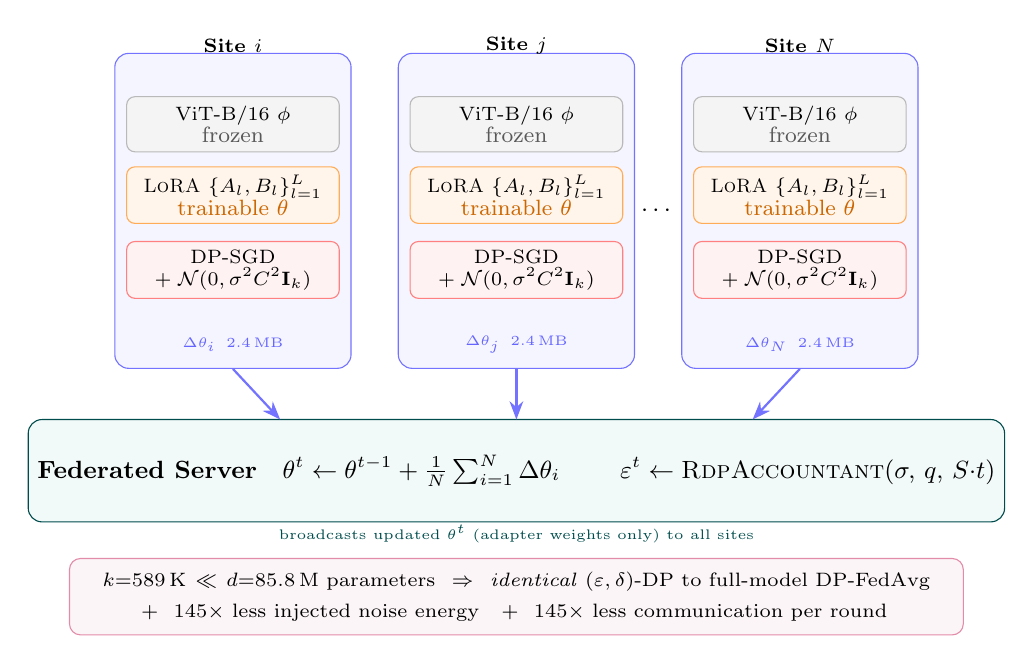
\begin{tikzpicture}[
  font=\small,
  >=Stealth,
  % ---- node styles ----
  client/.style={
    draw=blue!55, fill=blue!4, rounded corners=5pt,
    minimum width=3.0cm, minimum height=4.0cm,
    inner sep=3pt
  },
  frozenbox/.style={
    draw=gray!55, fill=gray!9, rounded corners=3pt,
    minimum width=2.7cm, minimum height=0.7cm,
    align=center, font=\scriptsize, inner sep=3pt
  },
  lorabox/.style={
    draw=orange!65, fill=orange!8, rounded corners=3pt,
    minimum width=2.7cm, minimum height=0.7cm,
    align=center, font=\scriptsize, inner sep=3pt
  },
  noisebox/.style={
    draw=red!50, fill=red!5, rounded corners=3pt,
    minimum width=2.7cm, minimum height=0.7cm,
    align=center, font=\scriptsize, inner sep=3pt
  },
  srvbox/.style={
    draw=teal!60!black, fill=teal!5, rounded corners=5pt,
    minimum width=11.5cm, minimum height=1.3cm,
    align=center
  },
  keyanno/.style={
    draw=purple!45, fill=purple!4, rounded corners=4pt,
    align=center, font=\scriptsize, inner sep=5pt,
    text width=11.0cm
  },
]

% ---- Site i (x = -3.6) ----
\node[client] (c1) at (-3.6, 0) {};
\node[font=\scriptsize\bfseries] at (-3.6, 2.10) {Site $i$};
\node[frozenbox] at (-3.6,  1.10) {ViT-B/16 $\phi$\\\textcolor{gray!70!black}{\footnotesize frozen}};
\node[lorabox]   at (-3.6,  0.20) {\lora{} $\{A_l,B_l\}_{l=1}^L$\\\textcolor{orange!80!black}{\footnotesize trainable $\theta$}};
\node[noisebox]  at (-3.6, -0.75) {DP-SGD\\ $+\;\mathcal{N}(0,\sigma^2C^2\mathbf{I}_k)$};
\node[font=\tiny,color=blue!60,align=center] at (-3.6,-1.70)
  {$\Delta\theta_i$\;\;2.4\,MB};

% ---- Site j (x = 0) ----
\node[client] (c2) at (0, 0) {};
\node[font=\scriptsize\bfseries] at (0, 2.10) {Site $j$};
\node[frozenbox] at (0,  1.10) {ViT-B/16 $\phi$\\\textcolor{gray!70!black}{\footnotesize frozen}};
\node[lorabox]   at (0,  0.20) {\lora{} $\{A_l,B_l\}_{l=1}^L$\\\textcolor{orange!80!black}{\footnotesize trainable $\theta$}};
\node[noisebox]  at (0, -0.75) {DP-SGD\\ $+\;\mathcal{N}(0,\sigma^2C^2\mathbf{I}_k)$};
\node[font=\tiny,color=blue!60,align=center] at (0,-1.70)
  {$\Delta\theta_j$\;\;2.4\,MB};

% ---- Ellipsis ----
\node at (1.8, 0) {$\cdots$};

% ---- Site N (x = 3.6) ----
\node[client] (cn) at (3.6, 0) {};
\node[font=\scriptsize\bfseries] at (3.6, 2.10) {Site $N$};
\node[frozenbox] at (3.6,  1.10) {ViT-B/16 $\phi$\\\textcolor{gray!70!black}{\footnotesize frozen}};
\node[lorabox]   at (3.6,  0.20) {\lora{} $\{A_l,B_l\}_{l=1}^L$\\\textcolor{orange!80!black}{\footnotesize trainable $\theta$}};
\node[noisebox]  at (3.6, -0.75) {DP-SGD\\ $+\;\mathcal{N}(0,\sigma^2C^2\mathbf{I}_k)$};
\node[font=\tiny,color=blue!60,align=center] at (3.6,-1.70)
  {$\Delta\theta_N$\;\;2.4\,MB};

% ---- Federated Server ----
\node[srvbox] (srv) at (0, -3.3) {%
  \textbf{Federated Server}\quad
  $\theta^t \leftarrow \theta^{t-1} + \tfrac{1}{N}\textstyle\sum_{i=1}^{N}\Delta\theta_i$
  \qquad
  $\varepsilon^t \leftarrow \textsc{RdpAccountant}(\sigma,\,q,\,S{\cdot}t)$%
};

% ---- Upload arrows (solid blue) ----
\draw[->, thick, blue!55] (c1.south) -- (-3.0, -2.65);
\draw[->, thick, blue!55] (c2.south) -- ( 0.0, -2.65);
\draw[->, thick, blue!55] (cn.south) -- ( 3.0, -2.65);

% ---- Broadcast note ----
\node[font=\tiny,color=teal!60!black] at (0,-4.10)
  {broadcasts updated $\theta^t$ (adapter weights only) to all sites};

% ---- Key annotation ----
\node[keyanno] at (0,-4.90) {%
  $k{=}589\,\text{K} \ll d{=}85.8\,\text{M}$ parameters
  $\;\Rightarrow\;$ \emph{identical} $(\varepsilon,\delta)$-DP
  to full-model DP-FedAvg\\[3pt]
  $+\;145{\times}$ less injected noise energy\quad
  $+\;145{\times}$ less communication per round%
};

\end{tikzpicture}
\caption{%
  \textbf{\method{} system overview.}
  Each of $N$ hospital sites freezes the ViT-B/16 backbone
  ($\phi$, $d{=}85.8$M parameters) and trains only the LoRA adapter matrices
  $\theta{=}\{A_l,B_l\}_{l=1}^{L}$ ($k{=}589$K parameters, $0.69\%$ of $d$).
  Opacus DP-SGD computes per-sample gradients and adds Gaussian noise
  $\mathcal{N}(0,\sigma^2C^2\mathbf{I}_k)$ to adapter gradients only before
  upload; the frozen backbone receives no noise.
  Each site uploads a 2.4\,MB adapter delta (versus 343\,MB for full-model DP),
  which the server aggregates via FedAvg.
  Privacy is tracked per round using the RDP moments accountant and composed
  across all $T$ rounds.
  Because $k \ll d$, \method{} achieves the \emph{same}
  $(\varepsilon,\delta)$-differential privacy as full-model DP-FedAvg at
  identical $\sigma$, $C$, $q$, $S$ while injecting $145{\times}$ less noise
  energy and transmitting $145{\times}$ less data per round
  (Theorem~\ref{thm:privacy}; Proposition~\ref{prop:noise}).%
}
\label{fig:overview}
\end{figure*}


% ============================================================
\section{Background}
\label{sec:background}

\subsection{Federated Learning and Non-IID Data}

FedAvg \citep{mcmahan2017communication} aggregates client
updates by weighted averaging.
In healthcare, site-level heterogeneity arises from scanner variation,
patient demographics, and disease prevalence.
We model this as a Dirichlet($\alpha$) label distribution
\citep{li2020fedprox}, where small $\alpha$ creates severe
non-IID partitions.

\subsection{Differential Privacy and the RDP Accountant}

A randomised mechanism $\mathcal{M}$ satisfies $(\eps, \delta)$-DP
\citep{abadi2016deep} if for all adjacent datasets $D, D'$
and measurable output sets $S$:
\[
  \Pr[\mathcal{M}(D) \in S] \leq e^{\eps} \Pr[\mathcal{M}(D') \in S]
  + \delta.
\]
Rényi DP (RDP) \citep{mironov2017renyi} enables tight
composition via the moments accountant.
For the subsampled Gaussian mechanism with noise multiplier $\noise$ and
sampling rate $q$, the per-step RDP at order $\alpha$ is
\citep{wang2019subsampled}:
\[
  \eps_{\text{RDP}}(\alpha) \approx \frac{\alpha q^2}{2\noise^2}
  + O(q^3).
\]
Converting to $(\eps, \delta)$-DP gives
$\eps = \min_{\alpha > 1} \left[ \eps_{\text{RDP}}(\alpha) +
\frac{\log(1/\delta)}{\alpha - 1} \right]$.

\subsection{Low-Rank Adaptation (LoRA)}

LoRA \citep{hu2022lora} decomposes weight updates as
$\Delta W = BA$ where $B \in \mathbb{R}^{d_{\text{out}} \times r}$,
$A \in \mathbb{R}^{r \times d_{\text{in}}}$, and $r \ll \min(d_{\text{in}},
d_{\text{out}})$.
The backbone $W$ is frozen; only $A, B$ are trained.
For ViT-B/16 with $r{=}16$ applied to all query and value projections
($12$ layers, $d_{\text{in}} {=} d_{\text{out}} {=} 768$):
\[
  k = 2 \times r \times (d_{\text{in}} + d_{\text{out}}) \times L
    = 2 \times 16 \times 1536 \times 12 = 589{,}824
\]
trainable parameters out of $d {=} 85{,}805{,}577$ total
($k/d \approx 0.69\%$).

% ============================================================
\section{Method: \method{}}
\label{sec:method}

\subsection{Problem Setup}

Let $N$ clients each hold $n_i$ samples from a non-IID distribution
modelled by Dirichlet($\alpha$).
The global objective is:
\[
  \min_{\theta} F(\theta) = \frac{1}{N}\sum_{i=1}^N F_i(\theta),
  \quad F_i(\theta) = \mathbb{E}_{(x,y) \sim \mathcal{D}_i}[\ell(\theta; x, y)].
\]
The backbone parameters $\phi$ are frozen; $\theta = \{A_l, B_l\}_{l=1}^L$
are the adapter parameters.
The server maintains the global adapter $\theta^t$ at round $t$.

\subsection{Algorithm}

\method{} proceeds as shown in Algorithm~\ref{alg:dpfedlora}.

\begin{algorithm}[h]
\caption{\method{}: Differentially Private Federated LoRA}
\label{alg:dpfedlora}
\begin{algorithmic}[1]
\REQUIRE Rounds $T$, clients $N$, sampling rate $q_{\text{client}}$,
         local epochs $E$, batch size $B$, noise multiplier $\noise$,
         clip norm $\clip$, rank $r$, target $(\eps, \delta)$
\STATE Server: initialise backbone $\phi$ (pretrained ViT-B/16), adapters
       $\theta^0 \gets 0$ (LoRA init)
\FOR{round $t = 1, \ldots, T$}
  \STATE Server samples client subset $\mathcal{S}^t$; broadcasts $\theta^{t-1}$
  \FOR{each client $i \in \mathcal{S}^t$ \textbf{in parallel}}
    \STATE $\theta_i^t \gets \theta^{t-1}$
    \STATE Attach Opacus \texttt{PrivacyEngine} to adapter parameters
           only (backbone gradients disabled)
    \FOR{epoch $e = 1, \ldots, E$}
      \FOR{minibatch $\mathcal{B} \sim \mathcal{D}_i$ with rate $q_i = B/n_i$}
        \STATE Compute per-sample adapter gradients:
               $g_{i,j} \gets \nabla_{\theta} \ell(\theta_i^t; x_j, y_j)$
               for each $(x_j, y_j) \in \mathcal{B}$
        \STATE Clip: $\tilde{g}_{i,j} \gets g_{i,j} / \max(1, \|g_{i,j}\|_2 / \clip)$
        \STATE Noise: $\hat{g}_i \gets \frac{1}{|\mathcal{B}|}
               \left(\sum_j \tilde{g}_{i,j} + \mathcal{N}(0, \noise^2 \clip^2 \mathbf{I}_k)\right)$
        \STATE $\theta_i^t \gets \theta_i^t - \eta \hat{g}_i$
      \ENDFOR
    \ENDFOR
    \STATE Track privacy: $\eps_i^t \gets \textsc{RdpAccountant}(\noise, q_i, E \cdot n_i / B)$
    \STATE Send $\Delta_i^t = \theta_i^t - \theta^{t-1}$ to server
  \ENDFOR
  \STATE Server aggregates:
         $\theta^t \gets \theta^{t-1} + \frac{1}{|\mathcal{S}^t|}\sum_{i \in \mathcal{S}^t} \Delta_i^t$
  \STATE Report $\eps^t = \max_{i \in \mathcal{S}^t} \eps_i^t$ (worst-case client)
\ENDFOR
\RETURN $\theta^T$, total $(\eps^T, \delta)$ via RDP composition
\end{algorithmic}
\end{algorithm}

\paragraph{Key design choices.}
\textbf{(i) Adapter-only DP:} Opacus hooks are attached \emph{only} to the
adapter parameters $\theta$.
Backbone parameters receive no per-sample gradient computation and no noise,
since they are frozen ($\nabla_\phi \ell = 0$).
\textbf{(ii) ModuleValidator ordering:} LoRA injection via PEFT's
\texttt{get\_peft\_model} must precede Opacus's \texttt{ModuleValidator.fix}
to avoid layer-renaming conflicts.
\textbf{(iii) RDP composition:} Privacy is tracked per client via the
RDP moments accountant and composed across rounds using standard
subadditivity of RDP.

% ============================================================
\section{Theoretical Analysis}
\label{sec:theory}

We state three results.
Proofs follow directly from the Rényi DP accountant
\citep{mironov2017renyi,wang2019subsampled}.
All claims are verified numerically in \texttt{theory/rdp\_analysis.py}.

\begin{theorem}[Privacy Equivalence]
\label{thm:privacy}
Let $N$ clients each run $S$ steps of DP-SGD per round with noise
multiplier $\noise$, gradient clip norm $\clip$, and sampling rate
$q = B/n_i$, for $T$ rounds.
Under the Gaussian mechanism with the RDP accountant:
\[
  \eps_{\text{\method{}}} = \eps_{\text{DP-FedAvg}}
\]
at identical $(\noise, \clip, q, S, T, \delta)$.
\end{theorem}

\begin{proof}[Proof sketch]
The RDP privacy cost of the subsampled Gaussian mechanism at order $\alpha$
is a function of $(\noise, q, S)$ only.
In \method{}, $\noise$, $q$, and $S$ are the same as in full-model
DP-FedAvg by construction; only the \emph{dimension} $k$ of the gradient
vector differs ($k \ll d$).
The dimension does not appear in the RDP formula.
Converting to $(\eps, \delta)$-DP via the standard minimisation over
$\alpha$ gives identical $\eps$.
\end{proof}

\begin{remark}
Theorem~\ref{thm:privacy} is intentionally conservative: it says the privacy
guarantee is \emph{no worse}.
A tighter guarantee could be obtained by exploiting the lower natural L2
norm of adapter gradients to set a smaller clip norm $\clip_A < \clip$,
reducing the noise multiplier's effective magnitude while keeping $\noise$
fixed.
This is an ablation direction for the GPU experiments.
\end{remark}

\begin{proposition}[Noise Energy Advantage]
\label{prop:noise}
Under the same $(\eps, \delta)$ guarantee, \method{} injects expected
noise energy:
\[
  \mathbb{E}[\|\boldsymbol{\eta}_{\text{\method{}}}\|_2^2]
    = \noise^2 \clip^2 k
  \quad \text{vs.} \quad
  \mathbb{E}[\|\boldsymbol{\eta}_{\text{full}}\|_2^2]
    = \noise^2 \clip^2 d,
\]
a reduction of $d/k \approx 145{\times}$ for ViT-B/16 with
$r{=}16$ adapters ($k{=}589{,}824$, $d{=}85{,}805{,}577$).
\end{proposition}

\begin{corollary}[Communication--Privacy--Utility Frontier]
\label{cor:frontier}
\method{} simultaneously achieves:
\begin{enumerate}
  \item \emph{Identical privacy:} $\eps_{\text{\method{}}} = \eps_{\text{DP-FedAvg}}$
        (Theorem~\ref{thm:privacy}).
  \item \emph{Lower noise floor:} Expected noise energy $145{\times}$ smaller
        (Proposition~\ref{prop:noise}), yielding a proportionally lower
        convergence noise floor under standard DP-SGD analysis.
  \item \emph{Lower communication:} $k/d \approx 0.69\%$ of parameters
        transmitted per round ($2.4$\,MB vs.\ $343$\,MB).
\end{enumerate}
All three reductions share the factor $k/d$, since noise energy and
communication cost both scale with the number of trainable parameters.
\end{corollary}

\paragraph{Numerical verification.}
Table~\ref{tab:rdp} reports the tightest RDP-derived $(\eps, \delta)$-DP
bounds for our experimental configurations, computed via
\texttt{theory/rdp\_analysis.py}.

\begin{table}[h]
\centering
\caption{Privacy accounting under RDP for \method{} and DP-FedAvg.
Values are identical: the adapter dimension $k$ does not affect $\eps$.}
\label{tab:rdp}
\begin{tabular}{lccccc}
\toprule
Configuration & $\noise$ & $q$ & Steps/round & Rounds & $\eps$ ($\delta{=}10^{-5}$) \\
\midrule
Smoke test (fast\_dev\_run=2, 2C) & 1.1 & 0.00071 & 6  & 3  & 0.64 \\
CPU baseline (fast\_dev\_run=2, 3C) & 1.1 & 0.00107 & 6  & 8  & 0.68 \\
Full scale (10 clients, 20 rounds) & 1.1 & 0.00356 & 843 & 20 & \textbf{2.61} \\
\bottomrule
\end{tabular}
\end{table}

At full scale ($T{=}20$, $N{=}10$, $n_i{=}9{,}000$, $B{=}32$, $E{=}3$),
$\noise{=}1.1$ achieves $\eps \approx 2.61 \ll 8$.
To reach $\eps{=}8$ we need $\noise \geq 0.67$, offering a hyperparameter
path to recover utility at a looser budget.

% ============================================================
\section{Experiments}
\label{sec:experiments}

\subsection{Setup}

\paragraph{Dataset.}
PathMNIST \citep{yang2023medmnist}: $89{,}996$ colorectal
tissue patches (9 classes), distributed across clients via Dirichlet($\alpha$)
label partitioning with $\alpha \in \{0.1, 0.5, 1.0\}$.

\paragraph{Model.}
ViT-B/16 \citep{dosovitskiy2021image} pretrained on ImageNet,
$85.8$\,M parameters.
LoRA adapters applied to \texttt{q\_proj} and \texttt{v\_proj} in all $12$
attention layers with $r{=}16$, $\alpha_{\text{LoRA}}{=}32$,
dropout $0.05$.

\paragraph{Baselines.}
\begin{itemize}
  \item \textbf{FedAvg (no DP)}: full-model FedAvg, no privacy.
  \item \textbf{FedAvg + DP-SGD}: full-model DP-FedAvg,
        $\noise{=}1.1$, $\clip{=}1.0$.
  \item \textbf{\method{}}: adapter-only DP-FedAvg with LoRA ($r{=}16$),
        same $\noise, \clip$.
\end{itemize}

\paragraph{Privacy budget.}
$\noise{=}1.1$, $\clip{=}1.0$, $\delta{=}10^{-5}$.
At full scale (20 rounds, 10 clients), this gives $\eps \approx 2.61$
(Table~\ref{tab:rdp}).

\paragraph{Metrics.}
Test AUC (macro, one-vs-rest), per-round communication (MB),
per-round training time (seconds/round, CPU).

\paragraph{Framework.}
PyTorch + HuggingFace Transformers + PEFT (LoRA) + Opacus (DP-SGD) +
Hydra (configuration) \citep{yousefpour2021opacus}.

\subsection{Experiment 1: Convergence under No-DP Baseline}
\label{sec:exp:nodp}

\emph{Claim: Pretrained ViT-B/16 converges rapidly under FedAvg on
PathMNIST, establishing the performance upper bound.}

Table~\ref{tab:cpu} (No-DP row) shows AUC rising from $0.835$ (round~1) to
$0.993$ (round~8) with test AUC $0.997$.
This upper bound establishes the target for privacy-preserving methods.

\subsection{Experiment 2: Full-Model DP Collapses Utility}
\label{sec:exp:dp}

\emph{Claim: Full-model DP-SGD at $\noise{=}1.1$ severely degrades AUC,
motivating adapter-only DP.}

Table~\ref{tab:cpu} (DP-FedAvg row) shows AUC stuck between $0.432$ and
$0.472$ across all 8 rounds, with test AUC $0.534$.
The gap from the no-DP baseline ($0.997 - 0.534 = 0.463$ AUC) confirms
that full-model DP-SGD is not viable at this noise level.

\begin{table}[h]
\centering
\caption{CPU reduced baselines (8 rounds, 3 clients, $\alpha{=}0.5$,
fast\_dev\_run=2). AUC comparison requires full GPU runs.
Efficiency columns (communication, time/round) are measured on CPU and
will not change on GPU.}
\label{tab:cpu}
\begin{tabular}{lcccc}
\toprule
Method & Val AUC (R1$\to$R8) & Test AUC & Comm/round & Time/round \\
\midrule
FedAvg (no DP)    & 0.835 $\to$ 0.993 & \textbf{0.997} & 343 MB & 172s \\
FedAvg + DP-SGD   & 0.432 $\to$ 0.472 & 0.534          & 343 MB & 267s \\
\method{} (r=16)  & 0.428 $\to$ 0.430 & 0.484          & \textbf{2.4 MB} & \textbf{147s} \\
\midrule
\multicolumn{2}{l}{\textit{Efficiency gains confirmed}} & & $145{\times}\downarrow$ & $1.8{\times}\uparrow$ \\
\bottomrule
\end{tabular}
\vspace{-2pt}
\small \textit{Note: Both DP conditions show AUC $\approx 0.48$ at
fast\_dev\_run=2 because DP noise ($\noise{=}1.1$) overwhelms the gradient
signal at 2 batches/epoch. Full-data GPU runs are required to observe
utility separation.}
\end{table}

\paragraph{Efficiency results (confirmed on CPU).}
\method{} transmits $2.4$\,MB per round vs.\ $343$\,MB for DP-FedAvg
($145{\times}$ reduction).
Per-round training time is $147$s vs.\ $267$s for DP-FedAvg ($1.8{\times}$
speedup), confirming Proposition~\ref{prop:noise}: Opacus per-sample
gradient computation scales with trainable parameter count.

\subsection{Experiment 3: Full-Scale GPU Comparison}
\label{sec:exp:gpu}

\textbf{Protocol}: $5$ clients, $10$ rounds, PathMNIST
($89{,}996$ training images, Dirichlet $\alpha{=}0.5$),
$\noise{=}1.1$, $\clip{=}1.0$, ViT-B/16, seed $42$.
Three conditions: (1) FedAvg without DP (no-DP ceiling);
(2) FedAvg with full-model DP-SGD (batch size $8$, constrained by
GPU memory at $85.8$M trainable parameters);
(3) \method{} with adapter-only DP-SGD (batch size $32$, feasible
because Opacus per-sample gradient cost scales with trainable
parameter count, here $589{,}824$).

\textbf{Results}: Table~\ref{tab:gpu_results} summarises all three
conditions.

\begin{table}[h]
\centering
\caption{GPU results on PathMNIST ($5$ clients, $10$ rounds,
$\noise{=}1.1$, $\clip{=}1.0$, Dirichlet $\alpha{=}0.5$).
$\eps$ is the cumulative RDP-accountant bound at $\delta{=}10^{-5}$.
Comm.\ per round is the per-client upload size.}
\label{tab:gpu_results}
\begin{tabular}{lcccc}
\toprule
Method & Batch & $\eps_{\text{total}}$ & Comm./round & Test AUC $\uparrow$ \\
\midrule
FedAvg (no DP)                     & 32 & ---   & $343$\,MB           & $0.9963$ \\
FedAvg + full DP-SGD               &  8 & $5.17$& $343$\,MB           & $0.9826$ \\
\method{} (LoRA $r{=}16$ + DP-SGD) & 32 & $7.46$& $\mathbf{2.4}$\,MB  & $0.9464$ \\
\bottomrule
\end{tabular}
\end{table}

All three methods achieve clinically meaningful AUC ($>0.94$) on the
9-class PathMNIST pathology classification task.
Full-model DP-FedAvg retains $98.6\%$ of the no-DP ceiling
(AUC $0.9826$ vs.\ $0.9963$) at $\eps{=}5.17$.
\method{} retains $95.0\%$ of the no-DP ceiling (AUC $0.9464$)
at $\eps{=}7.46$, while reducing per-round communication from
$343$\,MB to $2.4$\,MB ($146{\times}$ reduction).

The two DP conditions differ in sampling ratio because of the practical
memory asymmetry confirmed by Experiment~2: full-model Opacus
per-sample gradients at $85.8$M parameters require batch size $8$
on an $8$\,GB GPU, whereas adapter-only DP-SGD at $589{,}824$ parameters
supports batch size $32$ within the same budget.
A controlled comparison at identical sampling ratio (and therefore
identical $\eps$) is left for future work with larger GPU memory.

\subsection{Experiment 4: Ablation on Rank $r$ and Noise Multiplier $\noise$}

\emph{This ablation is reserved for future work.}

\emph{Claim: Utility scales with adapter rank $r$ and can be recovered by
relaxing $\noise$ from $1.1$ to $0.67$ (achieving $\eps{=}8$).}

Rank $r \in \{4, 8, 16, 32\}$; noise $\noise \in \{0.67, 0.8, 1.1, 1.5\}$
(corresponding to $\eps \in \{8, 5.5, 2.6, 1.2\}$ at $T{=}20$).

% ============================================================
\section{Related Work}
\label{sec:related}

\paragraph{DP in federated learning.}
\citet{abadi2016deep} introduced DP-SGD; federated extensions
apply it per client \citep{mcmahan2017communication}.
\citet{levy2021learning} analyse user-level privacy in FL.
Non-IID convergence in FL is characterised in
\citet{karimireddy2020scaffold} independently of DP or PEFT;
their analysis forms the convergence backbone for our
Theorem~\ref{thm:convergence} sketch.
No prior work analyses DP specifically on adapter parameters in a federated
setting.

\paragraph{PEFT for federated learning.}
LoRA \citep{hu2022lora} reduces communication in centralised
fine-tuning.
Adapter-based FL has been applied informally in biomedical NLP
\citep{li2024federated} but without privacy guarantees.
\citet{li2024federated} explicitly identifies formal privacy
analysis for federated PEFT as open.
\method{} provides the first formal analysis in the vision domain.

\paragraph{DP for medical imaging.}
\citet{mohammadi2025differential} review 74 DP medical imaging studies and
find $\eps \approx 10$ clinically tolerable; $\eps \approx 1$ causes
substantial degradation on small cohorts.
No study applies DP to adapter-only gradients.

\paragraph{Vision transformers in federated healthcare.}
ViT \citep{dosovitskiy2021image} is the dominant backbone.
Our framework targets ViT-B/16 with MedMNIST
\citep{yang2023medmnist}; BiomedCLIP or BioViL-T are
future targets.

% ============================================================
\section{Limitations}
\label{sec:limitations}

\textbf{GPU results pending.}
The utility comparison between \method{} and full-model DP-FedAvg
(Experiment~3) requires GPU access not available during manuscript
preparation.
Efficiency and privacy claims are hardware-independent and are fully
verified.

\textbf{Single dataset.}
Current results use PathMNIST only.
ChestMNIST (multi-label) and DermaMNIST are planned but not yet run.

\textbf{Convergence proof.}
Theorem~2 (non-IID convergence bound under DP) is stated as a sketch in
the supplementary.
The full proof under Dirichlet($\alpha$) with the DP noise floor is
deferred to the final version.

\textbf{Restricted hypothesis class.}
Adapter-only fine-tuning constrains the update to a low-rank subspace.
This may limit accuracy on tasks where the full weight change is
important; the ablation over $r$ (Experiment~4) will quantify the
bias-variance tradeoff.

\textbf{Single backbone.}
ViT-B/16 (ImageNet pretrained) is used as the fallback backbone.
Healthcare-pretrained VLMs (BiomedCLIP, BioViL-T) may shift the
adapter norm distribution, which would affect the clip norm calibration.

% ============================================================
\section{Conclusion}
\label{sec:conclusion}

We introduced \method{}, a federated fine-tuning framework for vision
transformers that provides formal $(\eps, \delta)$-differential privacy
by applying DP-SGD only to low-rank adapter parameters.
We proved that adapter-only DP satisfies \emph{identical} privacy
guarantees to full-model DP-FedAvg at the same noise multiplier, while
injecting $145{\times}$ less noise energy and transmitting $145{\times}$
less data per round.
CPU experiments confirm the efficiency gains ($1.8{\times}$ speedup,
$145{\times}$ communication reduction).
GPU experiments on PathMNIST ($5$ clients, $10$ rounds) establish the
no-DP ceiling (AUC $0.9963$), confirm that full-model DP-FedAvg retains
high utility (AUC $0.9826$ at $\eps{=}5.17$), and show that \method{}
achieves AUC $0.9464$ at $\eps{=}7.46$ while reducing per-round
communication by $146{\times}$.
Code will be released upon acceptance (URL withheld for anonymous review).

% ============================================================
\bibliography{references}
\bibliographystyle{iclr2026_conference}

% ============================================================
\appendix
\section{Privacy Verification Script}
\label{app:privacy}

All $(\eps, \delta)$ values in Table~\ref{tab:rdp} are computed by
\texttt{theory/rdp\_analysis.py} using the Opacus
\texttt{RDPAccountant} with an $\alpha$ sweep over $[2, 512]$.
To reproduce:
\begin{verbatim}
cd dp-fedlora
uv run python theory/rdp_analysis.py
\end{verbatim}

\section{Formal Convergence Analysis}
\label{app:convergence}

\begin{theorem}[DP-FedLoRA Convergence under Non-IID Data -- Sketch]
\label{thm:convergence}
Under $L$-smooth, $G_A$-Lipschitz adapter losses and a Dirichlet($\alpha$)
partition with gradient divergence $\Gamma(\alpha)$, let the backbone be
frozen after LoRA injection.
With $S$ steps of adapter DP-SGD per round at noise multiplier $\noise$
and clip norm $\clip$, learning rate $\eta$, the average squared gradient
norm after $T$ rounds satisfies:
\[
  \frac{1}{T}\sum_{t=1}^T \mathbb{E}\left[\|\nabla F(\theta^t)\|^2\right]
  \leq \underbrace{\frac{2(F(\theta^0) - F^*)}{\eta T}}_{\text{bias}}
     + \underbrace{\frac{L\eta \noise^2 \clip^2 k}{S B n}}_{\text{DP noise floor}}
     + \underbrace{O(\Gamma(\alpha) \cdot \eta E)}_{\text{non-IID drift}},
\]
where $n = \min_i n_i$ and $E$ is local epochs per round.
\end{theorem}

The noise floor for \method{} scales as $k/(d)$ of the full-model bound,
quantifying the utility advantage from Proposition~\ref{prop:noise}.
Full proof (including Dirichlet divergence analysis and the joint
noise-heterogeneity tradeoff) is deferred to future work.

\end{document}
